% ------------------------------------------------------------------------------
% TYPO3 CMS 6.2 LTS - What's New - Chapter "Introduction" (Italian Version)
%
% @author Roberto Torresani <roberto.torresani@typo3.org>
% @license	Creative Commons BY-NC-SA 3.0
% @link		http://typo3.org/download/release-notes/whats-new/
% @language	Italian
% ------------------------------------------------------------------------------
% Chapter: Introduction
% ------------------------------------------------------------------------------

\section{Introduzione}
\begin{frame}[fragile]
        \frametitle{Introduzione}

        \begin{center}\huge{Introduzione}\end{center}
        \begin{center}\huge{\color{typo3darkgrey}\textbf{(I fatti in breve)}}\end{center}

\end{frame}

% ------------------------------------------------------------------------------
% Standard Slide
% ------------------------------------------------------------------------------

\section{Introduzione}
\begin{frame}[fragile]
	\frametitle{Introduzione}
	\framesubtitle{TYPO3 CMS 6.2 LTS: Punti importanti}

	\begin{itemize}
		\item Focalizzata su:

			\begin{itemize}
				\item Gestione migrazione
				\item Fondamentale robustezza e sicurezza
				\item Felicità dell'utente
				\item Tecnologia e interazione moderna
			\end{itemize}

	\end{itemize}

	\begin{columns}[T]

		\begin{column}{.5\textwidth}
			\begin{itemize}
				\item Release Manager:
				\begin{itemize}
					\item Ernesto Baschny\newline
						ernesto.baschny (at) typo3.org\newline
						Twitter: @baschny
				\end{itemize}
			\end{itemize}
		\end{column}

		\begin{column}{.5\textwidth}
			\begin{figure}
				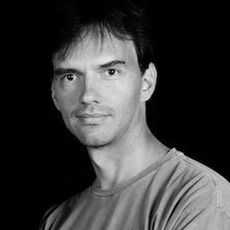
\includegraphics[width=2.6cm,height=2.6cm]{Images/Introduction/ErnestoBaschny.jpg}
			\end{figure}
		\end{column}

	\end{columns}

\end{frame}

% ------------------------------------------------------------------------------
% Standard Slide
% ------------------------------------------------------------------------------

\begin{frame}[fragile]
	% \TabPositions{1.2cm}

	\frametitle{Introduzione}
	\framesubtitle{TYPO3 CMS 6.2 LTS: Punti importanti}

	\begin{itemize}
		\item Data di rilascio: 25 Marzo 2014
		\item Tempi dello sviluppo e dei rilasci:
	\end{itemize}

	\begin{figure}
		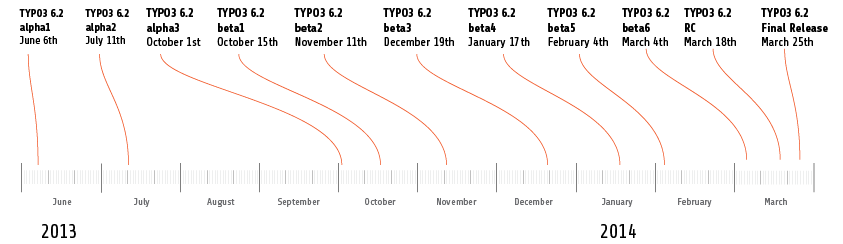
\includegraphics[width=0.99\linewidth]{Images/Introduction/ReleaseTimeline.png}
	\end{figure}

\end{frame}

% ------------------------------------------------------------------------------
% Standard Slide
% ------------------------------------------------------------------------------

\begin{frame}[fragile]
	\frametitle{Introduzione}
	\framesubtitle{TYPO3 CMS 6.2 LTS: Punti importanti}

	\begin{itemize}
		\item Requisiti di sistema
		\begin{itemize}
			\item PHP	\tabto{1.2cm} v5.3.7 - v5.5.x
			\item MySQL	\tabto{1.2cm} v5.1.x - v5.6.x
		\end{itemize}
	\end{itemize}

	\begin{itemize}
		\item Fine del mantenimento: 30 Dicembre 2016
		\item TYPO3 CMS 6.2 è una versione a  \textbf{Lungo Supporto} (LTS) (3 anni di supporto!)
	\end{itemize}

\end{frame}

% ------------------------------------------------------------------------------
% Standard Slide
% ------------------------------------------------------------------------------

\begin{frame}[fragile]
	\frametitle{Introduzione}
	\framesubtitle{TYPO3 CMS 6.2 LTS: Punti importanti}

	\begin{itemize}
		\item Agenda dei rilasci:
	\end{itemize}

	\begin{figure}
		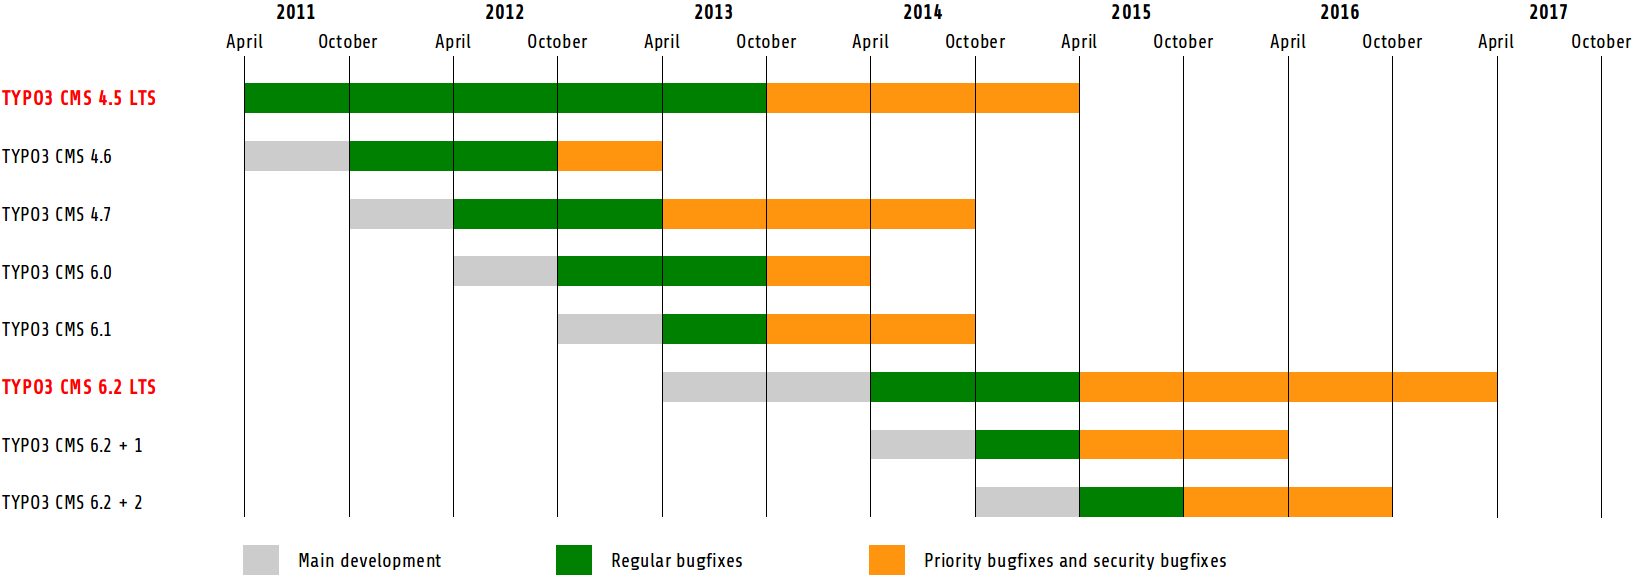
\includegraphics[width=0.99\linewidth]{Images/Introduction/ReleaseAgenda.png}
	\end{figure}

\end{frame}

% ------------------------------------------------------------------------------

